\chapter{Background}\label{chap:background}
This chapter explores various works done by the industry and researchers which acts as the basis for the later topics in the dissertation. 

\section{The Microservice Architecture}
Usually, a set of small loosely coupled components that can be deployed, scaled and tested independently which make up for a cloud-native application, more commonly known as the Microservice architecture. A major reason for the introduction of this architecture has been the ever-increasing demand for deploying cloud-native applications as various industries embrace a software-driven model. 

Using the microservice architecture comes with its own set of unique features, these features allow for new deployment patterns to be discussed and why this paper exists. 

Such features are listed below: 

\begin{itemize}
    \item Highly maintainable and testable 
    \item Loosely coupled with other services 
    \item Independently deployable 
    \item Capable of being deployed by a smaller team
\end{itemize}

\textbf{Why are microservice often used in industry now and what advantages do these have?}

\section{Deployment Patterns}
\textbf{WHY DO THESE PATTERNS MATTER?? }
% https://www.nginx.com/blog/deploying-microservices/
Microservice applications consist of multiple services, which are created using different technologies. Each service has specific run-time requirements, such as needing appropriate CPU, Memory and I/O resources, or requiring a certain number of instances for the service to keep up with demand. This means that deploying a microservice application can be challenging as the services should be able to deploy in a speedy, reliably and be cost-effective manner. 

The following patterns are set out to remedy issues with deploying services to the cloud, these can be used interchangeably if required. The patterns itself have been set out by the author of microservices.io, Chris Richardson \cite{Chr19}. 

\subsection{Pattern 1: Single application per machine}
    \begin{figure}[H]
        \centering
        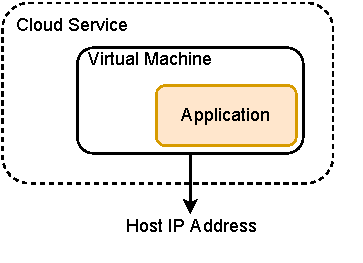
\includegraphics[width=0.45\linewidth]{images/Pattern-1.pdf}
        \caption{An example application is used for visualizing the pattern mentioned here.}
    \end{figure}  

A basic pattern in which a single microservice application is deployed on one machine allows for a simple and cost-effective deployment depending on the use-case scenario. The ideal scenario would fit an application with a small user-base however would see themselves grow within the future to utilize the various advantages of the microservice architecture \cite{Chr19}.. 

\subsection{Pattern 2 : Multiple service instance per multiple hosts}
    \begin{figure}[H]
        \centering
        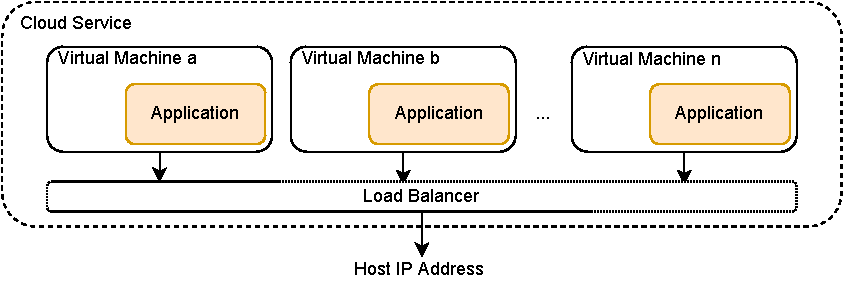
\includegraphics[width=0.9\linewidth]{images/Pattern-2.pdf}
        \caption{An example application is used for visualizing the pattern mentioned here.}
    \end{figure}  

\subsection{Pattern 3 : Single service instance per multiple hosts}
    \begin{figure}[H]
        \centering
        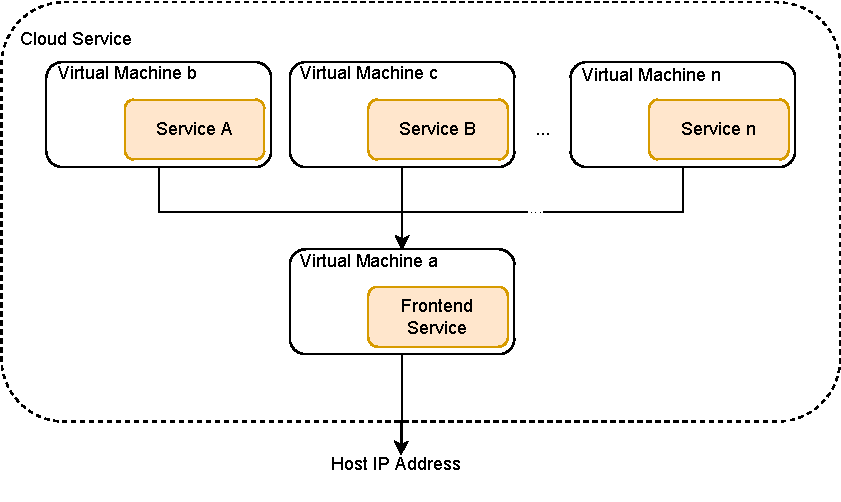
\includegraphics[width=0.8\linewidth]{images/Pattern-3.pdf}
        \caption{An example application is used for visualizing the pattern mentioned here.}
    \end{figure}  



\section{Azure}


\section{Infrastructure As A Platform -Terraform}
% https://amazicworld.com/building-auto-scaling-groupss-in-azure-with-terraform/

The Infrastructure as code platform used for the project is an open source tool developed by HashiCorp called Terraform, it uses a declarative language to deploy and manage infrastructure across a variety of cloud providers, private clouds and virtualization platforms. 


\subsection{Terraform Azure}
\begin{lstlisting}
    terraform {
      required_providers {
        azurerm = {
          source = "hashicorp/azurerm"
          version = "~>2.0"
        }
      }
    }
    
    # Use a pre-created resource group
    data "azurerm_resource_group" "{resource_name}" {
    	name = "{resource_name}"
    }
    
\end{lstlisting}

\subsection{Modules}
Modules are used to create light weight abstractions which can be used to describe infrastructure in terms of the architecture instead of fixed variable names. 
\subsubsection{Root Module}
\subsubsection{Child Modules}
